\chapter{Architettura e Design}
\label{ch:architectures}

\section{Design generale del software}

L'architettura del software è basata su micro-servizi autonomi e indipendenti tra loro e la loro comunicazione avviene tramite API REST.
Esiste un middleware che si occupa della gestione e dell'orchestrazione dei micro-servizi, facendo appunto da ponte collegando le varie diverse tencologie.

I microservizi che si sono scelti di sviluppare si occupano di varie aree legate alla natura del progetto e sono:
\begin{itemize}
    % \item \textbf{ChatService}: si occupa della gestione delle chat tra utenti.
    \item \textbf{UserService}: si occupa della gestione degli utenti, quindi la loro registrazione, autenticazione e gestione dei dati personali.
    \item \textbf{BusinessLogic}: si occupa di mantenere al proprio interno tutte le regole proprie del gioco
    \item \textbf{Front-End}: si occupa di gestire l'interfaccia grafica e la comunicazione con il middleware.
    \item \textbf{Middleware}: si occupa della gestione delle comunicazioni tra i vari microservizi, e svolge la funzione di "motore di gioco".
\end{itemize}

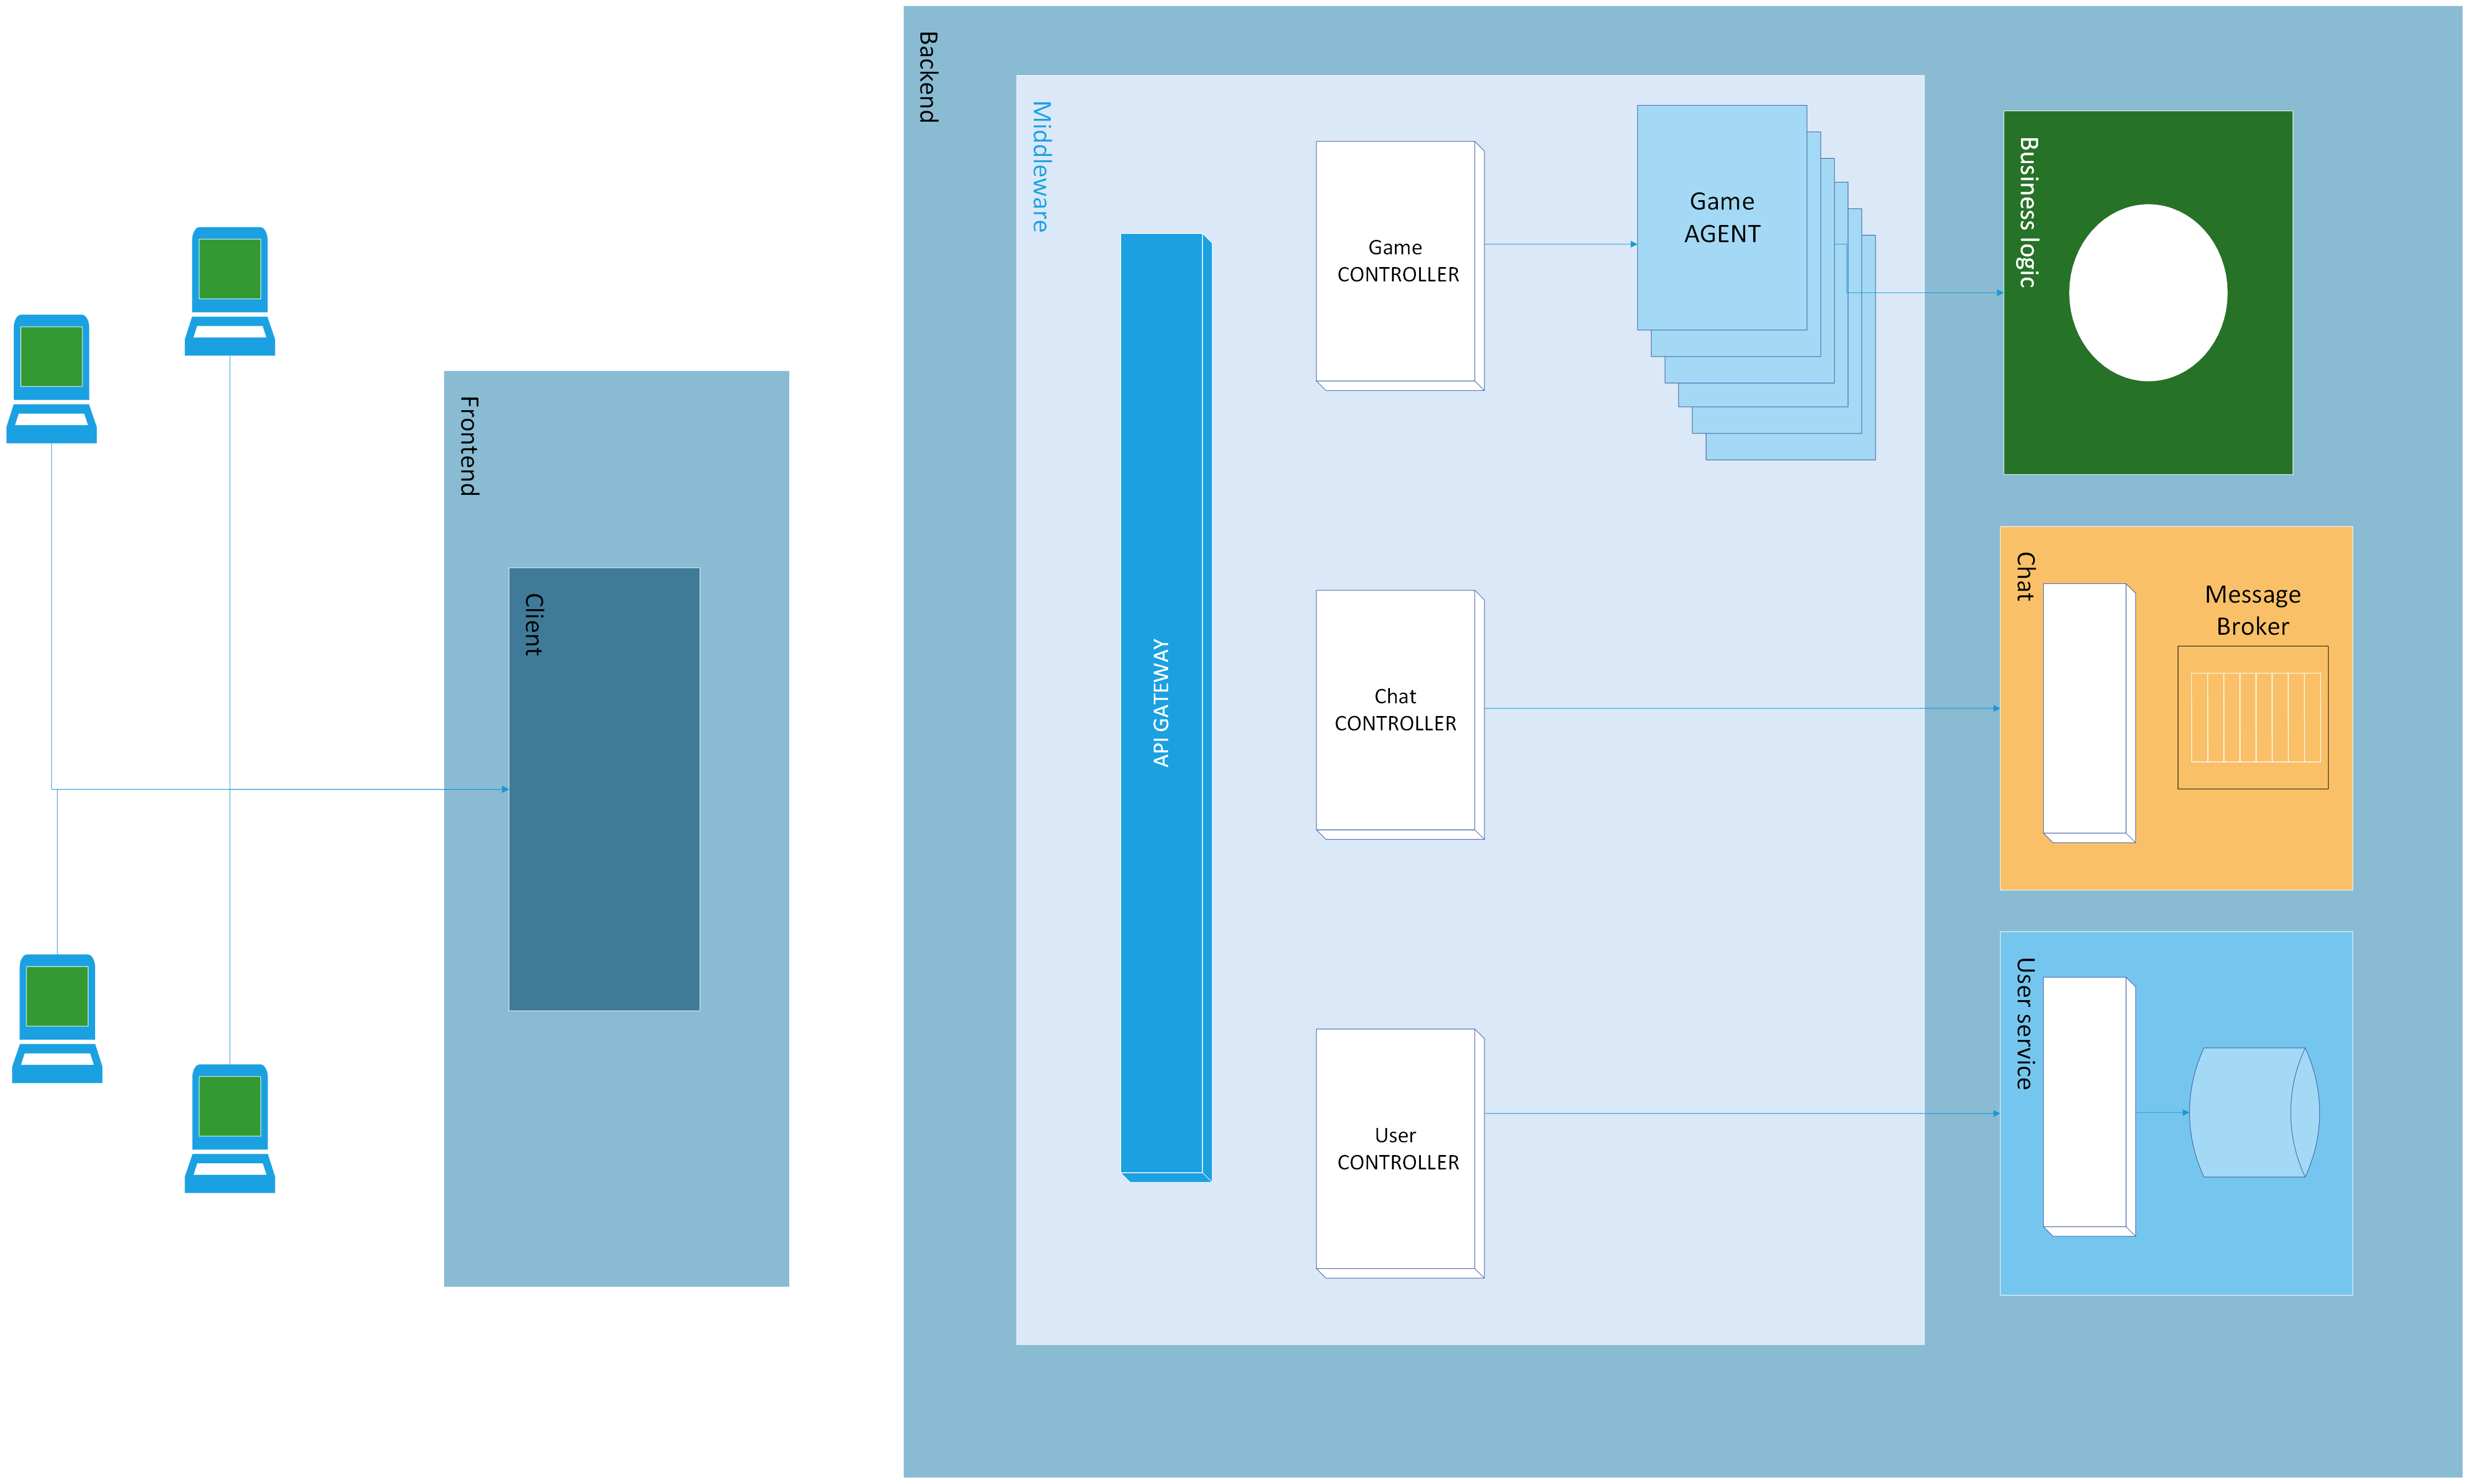
\includegraphics[width=12cm]{report/img/Architecture.png}\\[10.5cm]

\section{Micro-servizi e la loro architettura}

% \subsection{Servizio per la Chat}

% \begin{table}[h!]
%     \centering
%     \caption{Tabella descrittiva Chat Service}
%     \label{tab:chat_serv_table}
%     \begin{tabular}{ll}     
%         \toprule                   
%         Linguaggio & Java \\        
%         Server & Vertx, Swagger \\
%         Librerie & RabbitMQ(vertx) \\
%         Architettura & Agenti vertx \\
%         \bottomrule
%     \end{tabular}
% \end{table}

% 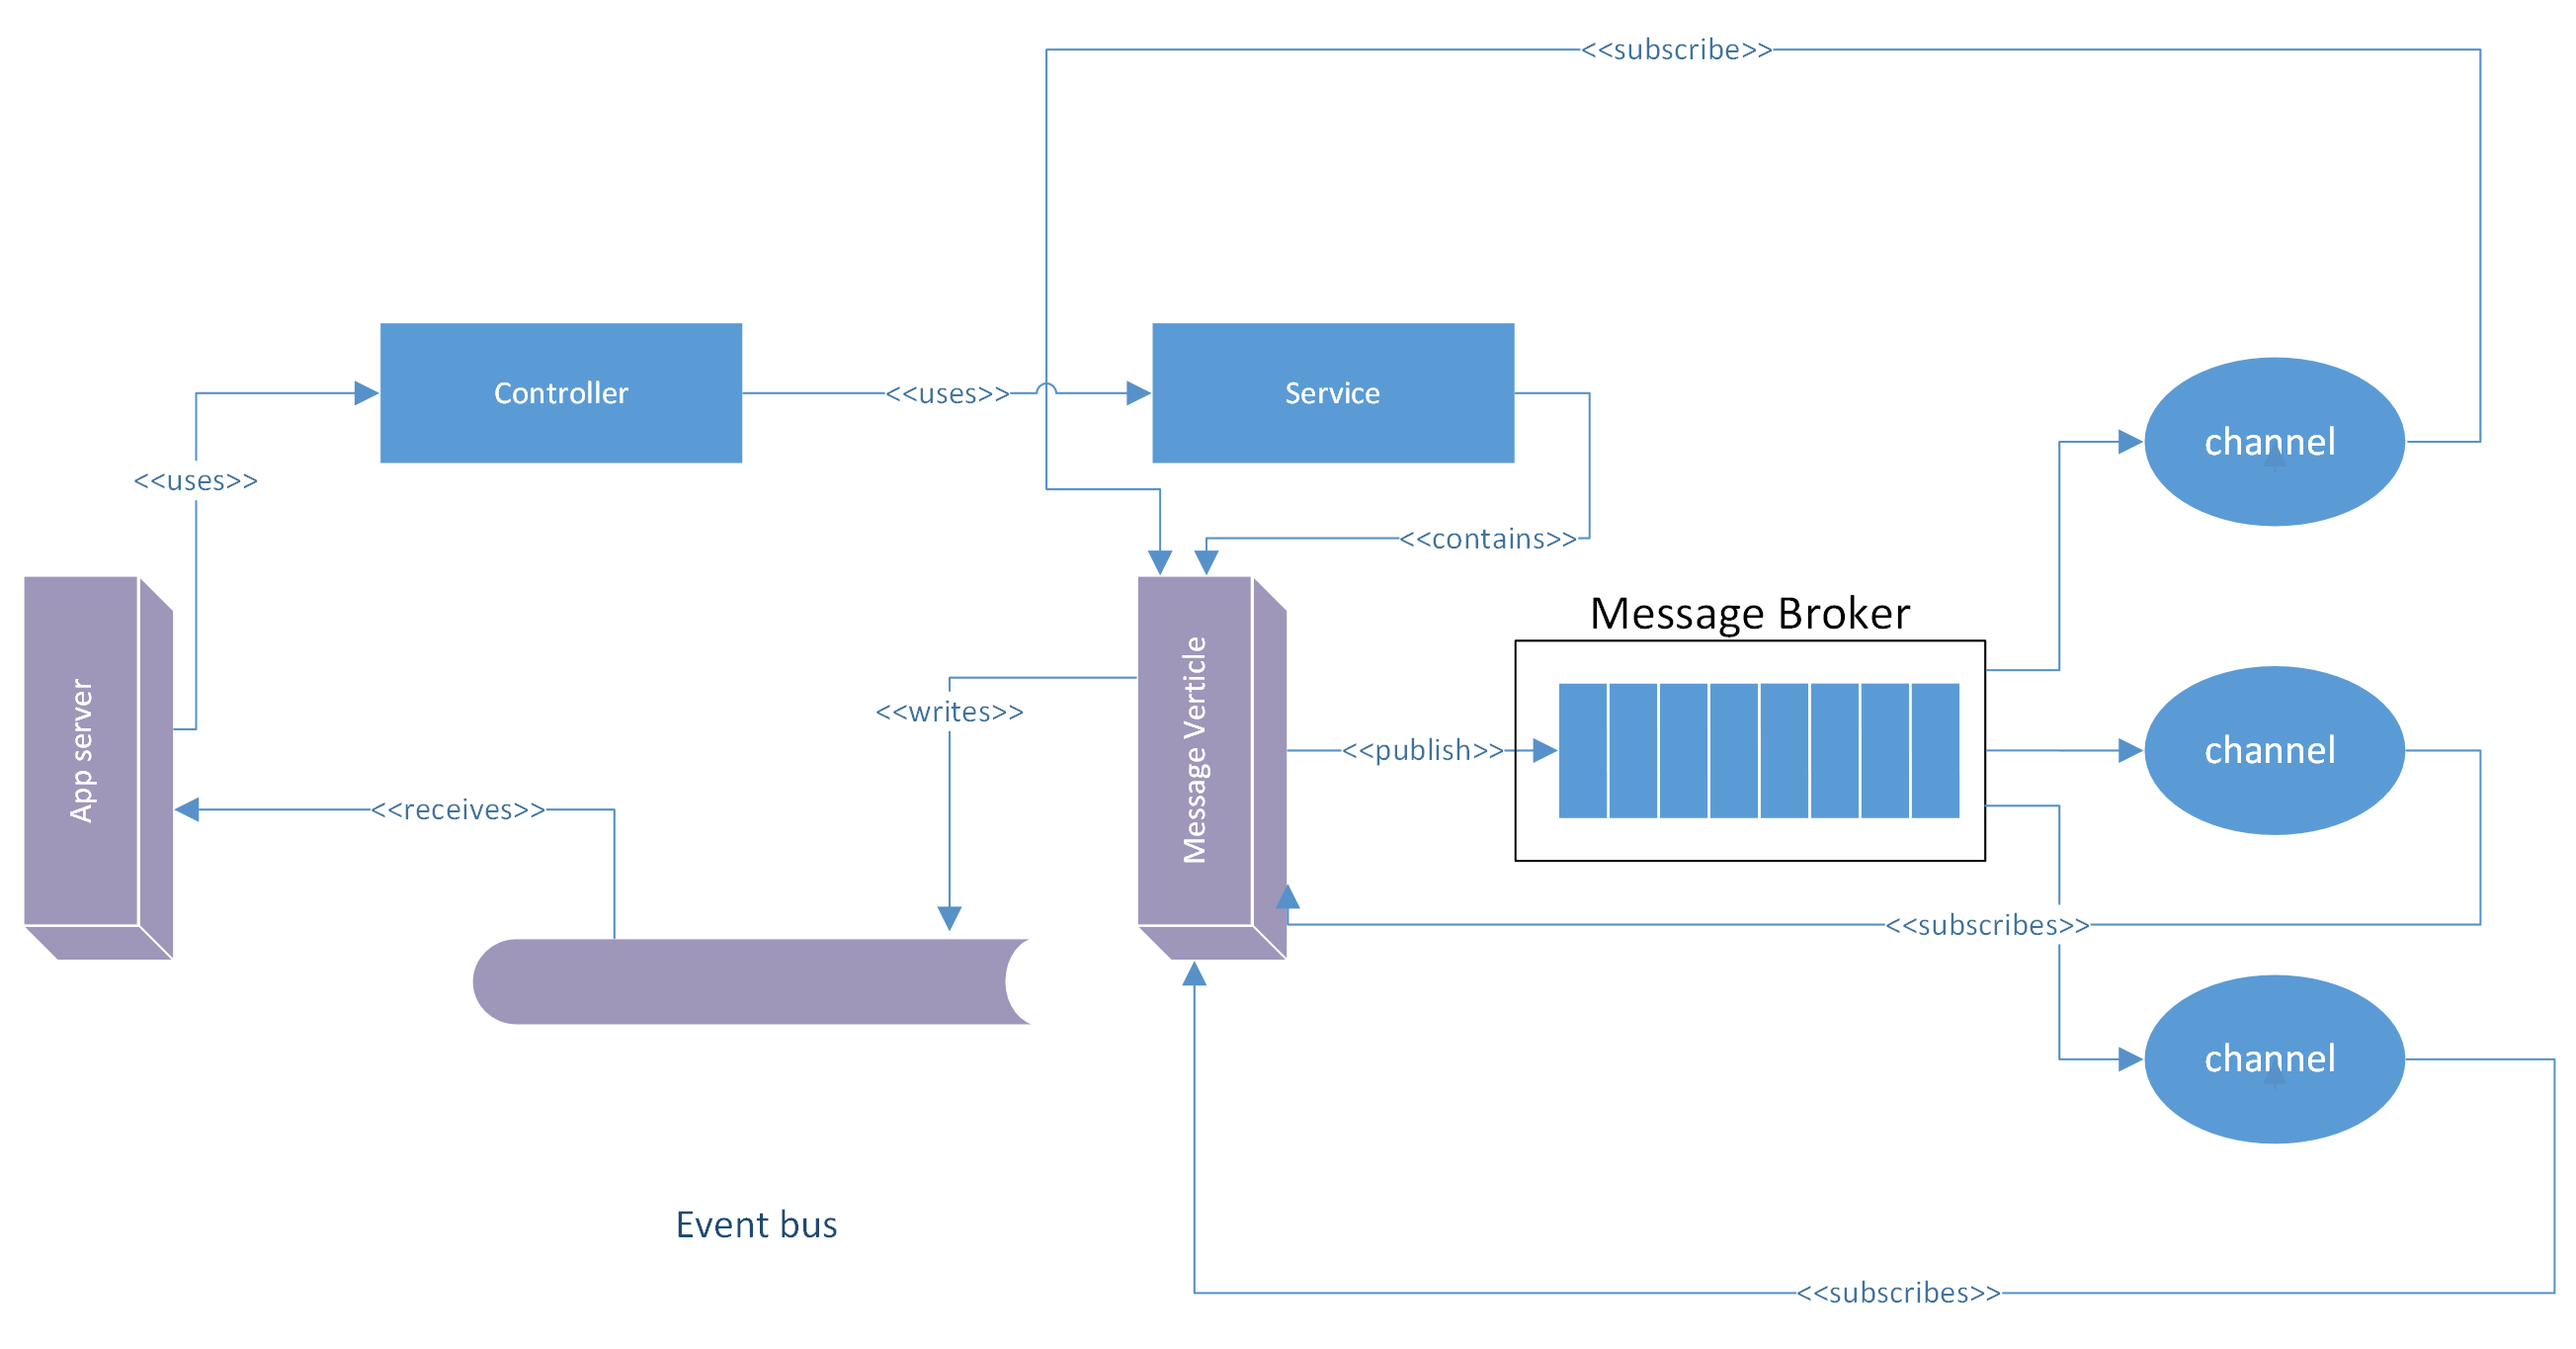
\includegraphics[width=15cm]{report/img/Architettura ChatService.png}\\[10.5cm]

\subsection{Servizio per Gestione Utenti}

\begin{table}[h!]
    \centering
    \caption{Tabella descrittiva User Service}
    \label{tab:user_serv_table}
    \begin{tabular}{ll}     
        \toprule                   
        Linguaggio & Node.JS/TypeScript \\        
        Framework & NestJS   \\                   
        Persistence & Mysql  \\
        Librerie & TypeORM   \\
        Architettura & Model-Controller-service  \\
        \bottomrule
    \end{tabular}
\end{table}


\subsection{Servizio Business Logic}

\begin{table}[h!]
    \centering
    \caption{Tabella descrittiva Business Logic}
    \label{tab:bl_serv_table}
    \begin{tabular}{ll}     
        \toprule                   
        Linguaggio & Node.JS/TypeScript \\        
        Framework & NestJS   \\                   
        Architettura & Model-Controller-service  \\
        \bottomrule
    \end{tabular}
\end{table}

\subsection{Servizio ponte tra i microservizi}


\begin{table}[h!]
    \centering
    \caption{Tabella descrittiva Middleware}
    \label{tab:middleware_serv_table}
    \begin{tabular}{ll}     
        \toprule                   
        Linguaggio & Java \\        
        Server & Vertx \\
        Librerie & RabbitMQ(vertx) \\
        Architettura & Multi-agent, motore di gioco \\
        \bottomrule
    \end{tabular}
\end{table}

\section{[DS/SPE] Perche' i microservizi?}

Ogni microservizio si occupa di gestire un singolo ambito di progetto, il che fa sì che si ottengano ottimi risultati riguardo la qualità e l'affidabilità, la riutilizzabilità, la flessibilità e la scalabilità.
Tutti i componenti sono "loosely coupled", distribuiti in modo indipendente, altamente collaudabili e gestibili e in ambiti reali gestiti da un piccolo team.
Tuttavia, non si tratta di una soluzione definitiva, ha anche degli svantaggi come ad esempio:
\begin{itemize}
    \item la complessità di gestione e la necessità di un'infrastruttura di rete molto complessa.
    \item un'ottima comunicazione di team.
    \item una discreta capacità di astrazione e progettazione di interfaccie di comunicazione che devono essere rispettate da tutti i microservizi.
    \item Non si ha la certezza che l'infrastruttura funzioni correttamente fino a quando tutti i servizi non cooperano tra loro.
\end{itemize}

% \subsection{[SPE] Vantaggi}
% - devops
% - ci 

\subsection{Vantaggi dell'architettura a microservizi}

\subsubsection{Fault Tolerance}

Progettare un sistema completamente privo di errori è un obiettivo decisamente ambizioso e molto difficile da raggiungere. 
Molto più realistico, e inerente al nostro percorso, è progettare un sistema che sia in grado di tollerare, nella giusta misura, gli errori che inevitabilmente si verificheranno. 
La scelta di questa architettura tra i vari vantaggi offre la possibilità di \textbf{isolare parti del sistema}, evitando che gli errori si propaghino in modo incontrollato e che il sistema nel suo complesso vada in crash. 
Ogni sistema opera in modo indipendente e autonomo, con le proprie risorse e la propria logica.
\vspace{1cm}

Lo snodo centrale di comunicazione dei servizi, il middleware, è in grado di gestire le comunicazioni tra i vari microservizi e di garantire che il sistema sia in grado di funzionare anche in caso di guasti.
Purtroppo non esiste alcun progetto senza alcun tipo di \textbf{single point of failure}, o almeno non con le risorse a disposizione di noi studenti, quindi all'interno di questo servizio la 
gestione degli errori dei servizi con cui comunica è gestita, ma di fatto, nel caso in cui il middleware smetta di funzionare, non avendo nessun altro servizio che possa fare da garante 
per il suo corretto funzionamento, tutto il sistema non permetterà, ad esempio, di giocare a nessun gioco.
Questo perché il middleware è il cuore pulsante del sistema; avendo disponibilità di risorse e abbastanza conoscenze in un ambito reale, questo problema ha soluzioni: 
\begin{itemize}
    \item \textbf{Backup del middleware}: avere dei backup dei processi che si occupano di gestire le partite, ma questo significherebbe andare a modificare inevitabilmente 
    la struttura già esistente del servizio.
    \item \textbf{Ridondanza del middleware}: avere molteplici istanze del middleware, preferibilmente 3, di cui una principale e le altre 2 in copia, facendo in modo che
    ogni azione sul middleware principale venga replicata sulle altre due istanze e che quindi, in caso di guasto hardware, le altre copie possano rispondere alle richieste.
\end{itemize}

\subsubsection{Scalabilità}

Nel caso del middleware, la scalabilità è un altro modo per chiamare la duplicazione, ma questo si applica soltanto al middleware, in quanto gli altri microservizi sono realmente scalabili.
Ogni microservizio è in grado di scalare in modo indipendente, in base alle proprie esigenze, e questo permette di avere un sistema che si adatta in modo dinamico alle richieste degli utenti. 
Nella prossima sezione verrà approfondito come il deployment con Docker permetta di scalare i microservizi. L'implementazione di un sistema di load balancing viene fornita
"gratuitamente" da Kubernetes, che permette di bilanciare il carico tra i vari nodi del cluster. 
Qualora il progetto maraffa-online dovesse avere un numero di utenti molto elevato, si potrebbe pensare di scalare il sistema in modo orizzontale, aggiungendo nuovi nodi al cluster, 
e tramite la dovuta configurazione, Kubernetes si occuperebbe di bilanciare il carico tra i vari nodi dei servizi scalabili. 


\subsubsection{Docker}

Suddividere un progetto monolitico in servizi a sé stanti permette di dockerizzare comodamente ogni servizio, e questo consente di avere un sistema facilmente deployabile, versionabile e portabile.
Uno dei requisiti fondamentali del progetto era riuscire a dockerizzare interamente il sistema. Nel caso in cui si volesse fare un deploy su un server remoto, sarebbe sufficiente avere Docker installato, accedere al docker-compose del progetto, settare le corrette variabili d'ambiente e poi il progetto opererebbe in totale autonomia.
Inoltre, utilizzare uno stack permette anche di gestire eventuali failure dei servizi in modo più semplice, poiché Docker consente di avere un sistema fault-tolerant. Se un servizio dovesse andare in crash per qualche motivo inspiegabile, Docker si occuperebbe di riavviarlo in modo autonomo.
L'utilizzo di uno stack permette anche di scalare i servizi in modo più semplice, poiché basta settare il numero di repliche desiderate per un servizio e Docker si occuperà di creare le repliche e di bilanciare il carico tra di esse. Questo è un vantaggio nel caso in cui si voglia scalare il sistema in modo verticale, ovvero aumentando le risorse di un singolo servizio.


\section{Servizi di Business Logic e User Service}

Entrambi questi servizi sono stati realizzati con lo stack NestJS, un framework per Node.js che semplifica la realizzazione di web server e API REST.
Si occupano rispettivamente di gestire la logica di gioco e la gestione degli utenti che vogliono utilizzare il sistema, due core business del progetto.

\subsection{Business Logic}

Questo servizio mantiene al proprio interno tutte le regole del gioco e il calcolo dei punteggi. 
Ha svariati endpoint che permettono al middleware di avere il minor numero possibile di responsabilità, delegando al servizio di business logic le operazioni riguardanti il gioco.

Questa scelta è stata fatta per mantenere il middleware il più leggero possibile e per evitare che si occupi di operazioni non di sua competenza. Inoltre, in futuro sarà possibile aggiungere nuovi giochi modificando il meno possibile il middleware, che dovrà semplicemente occuparsi della gestione delle partite e comunicare tempestivamente con i servizi di business logic in base al gioco scelto.

\subsection{User Service}

Questo servizio gestisce gli utenti, quindi la loro registrazione, autenticazione e gestione dei dati personali.
Anche in questo caso, il middleware delega al servizio di gestione degli utenti le operazioni riguardanti gli utenti, per mantenere il middleware il più leggero possibile e per evitare che si occupi di operazioni non di sua competenza.
Il core di questo servizio è dato dalla combinazione di NestJS e TypeORM, che permettono di gestire in modo semplice e veloce la persistenza dei dati e le operazioni CRUD su un database MySQL.
Oltre alle informazioni degli utenti, il database contiene anche le informazioni riguardanti le partite giocate e le statistiche personali di ogni utente del sistema.

\section{Front-End}

Il front-end è stato realizzato con Angular e si occupa di gestire l'interfaccia grafica e la comunicazione con il middleware.
Sono state realizzate diverse pagine, tra cui la home page, la pagina di registrazione, la pagina di login, la pagina di gioco e la pagina di profilo utente.
Utilizza API REST per comunicare con il middleware e ottenere i dati necessari per il funzionamento del gioco, mentre utilizza WebSockets per la comunicazione in tempo reale con il middleware. 

%TODO altro da dire sui servizi ?

\section{Middleware}

Come già citato, il middleware è il cuore del sistema. L'architettura utilizzata per la gestione delle partite è quella di un multi-agente, in cui ogni agente si occupa di gestire una partita 
e di orchestrare la comunicazione con gli altri servizi, come ad esempio il front-end. Questo core è stato realizzato con Vertx, che è stato utilizzato anche per creare un web-server in Java.

Inoltre, al middleware è collegato un database NoSQL su MongoDB, che viene aggiornato a ogni trick completato dai giocatori per creare uno storico delle partite e salvare le loro decisioni in gioco. 
Questa raccolta di dati sarà parte di uno sviluppo futuro, in cui, dopo aver raccolto una grande quantità di dati di partite, si potrà tentare di creare un modello di machine learning per sviluppare un'intelligenza artificiale che possa giocare al posto di un giocatore umano.

\subsection{Struttura API Gateway}

Il pattern di progettazione utilizzato per la realizzazione del middleware è quello dell'API Gateway, che permette di creare un'interfaccia unica per l'accesso ai vari servizi del sistema.

Nel nostro progetto, il client effettua semplici chiamate verso il middleware, che nei casi necessari effettua chiamate verso altri servizi per svolgere una determinata operazione.
Queste chiamate non sono obbligatoriamente dirette verso il servizio interessato, ma possono anche essere routine che effettuano molteplici chiamate per ottenere il risultato desiderato. 
Ad esempio, nel caso di una partita, considerando l'azione di giocare sul tavolo una carta da parte di un utente, il middleware si occuperà di effettuare alcune chiamate verso il servizio di business
logic per assicurarsi che la carta giocata in quel momento sia valida rispetto alle altre presenti sul tavolo virtuale e di conteggiare effettivamente i punti della mano nel caso in cui tutti i giocatori abbiano giocato una carta. Implementare queste chiamate direttamente nel front-end avrebbe reso il codice molto più complesso e difficile da mantenere, e la gestione di partite multiple sarebbe stata molto più difficile.

Non è stato implementato nessun meccanismo di discovery per la gestione di chiamate verso gli altri servizi, in quanto tutti presenti sullo stesso server e nello stesso stack di Docker, quindi facilmente individuabili sulla rete virtuale creata da Docker.

% \section{Punti comuni tra i servizi}

% \subsection{Swagger}